% =========================================================
% Các style TikZ dùng chung cho cả báo cáo
% =========================================================
\tikzset{
  block/.style     = {draw, rectangle, rounded corners=3pt, minimum width=2.2cm, minimum height=0.85cm, align=center, fill=blue!10, draw=blue!60, font=\small},
  io/.style        = {draw, trapezium, trapezium left angle=75, trapezium right angle=105, minimum width=2cm, minimum height=0.8cm, align=center, fill=green!10, draw=green!60!black, font=\small},
  decision/.style  = {draw, diamond, aspect=2.2, minimum width=2cm, minimum height=0.7cm, align=center, fill=orange!15, draw=orange!70, font=\scriptsize},
  arrow/.style     = {-{Stealth[length=2mm]}, draw=gray!70, thick},
  sarrow/.style    = {-{Stealth[length=2mm]}, draw=blue!50, thick, dashed},
  bus/.style       = {draw, rectangle, minimum width=4cm, minimum height=0.5cm, fill=gray!20, draw=gray!60, font=\tiny},
  chip/.style      = {draw, rectangle, rounded corners=2pt, minimum width=3cm, minimum height=1.2cm, align=center, fill=yellow!15, draw=orange!60, font=\small\bfseries},
  fpga/.style      = {draw, rectangle, rounded corners=5pt, minimum width=5.5cm, minimum height=3.5cm, align=center, fill=blue!5, draw=blue!50, very thick},
  signal/.style    = {draw=red!70, thick},
}

% =========================================================
% FINAL PROJECT  –  Trigonometric IP Core (CORDIC)
% =========================================================
\setcounter{section}{0}
\section{FINAL PROJECT: THIẾT KẾ IP THỰC HIỆN HÀM LƯỢNG GIÁC VỚI GIAO THỨC AVALON-MM}

\subsection{Trình bày, vẽ sơ đồ mạch theo cách hiểu của học viên}

\textbf{Mục tiêu:} Thiết kế một IP tùy chỉnh (Custom IP) thực hiện ba hàm lượng giác: $\sin$, $\cos$, $\tan$ sử dụng giao thức Avalon Memory-Mapped (Avalon-MM). Vi xử lý Nios II được kết nối và sử dụng như một công cụ quản lý dữ liệu, truyền dữ liệu đầu vào tới và nhận kết quả đầu ra từ IP lượng giác.

\textbf{Các cổng I/O:}
\begin{itemize}
    \item \textbf{Inputs:} Góc đầu vào $\theta$ được biểu diễn dưới dạng số nguyên 32-bit (Q16.16 fixed-point), tương ứng với góc tính bằng độ.
    \item \textbf{Outputs:} Kết quả của $\sin(\theta)$, $\cos(\theta)$ và $\tan(\theta)$ tương ứng, được trả về dưới dạng Q16.16 fixed-point.
\end{itemize}

\textbf{Phương pháp triển khai:} IP lượng giác được thiết kế sử dụng thuật toán CORDIC (COordinate Rotation DIgital Computer) -- một giải thuật hiệu quả về mặt phần cứng, chỉ cần phép dịch bit và phép cộng/trừ để tính toán các hàm lượng giác mà không cần nhân/chia. Độ chính xác được cải thiện bằng cách tăng số lần lặp CORDIC (16 vòng lặp với giá trị 32-bit).

Sơ đồ mạch thể hiện kiến trúc tổng thể của hệ thống SoC với IP lượng giác được tích hợp thông qua giao tiếp Avalon-MM:

\begin{figure}[H]
    \centering
    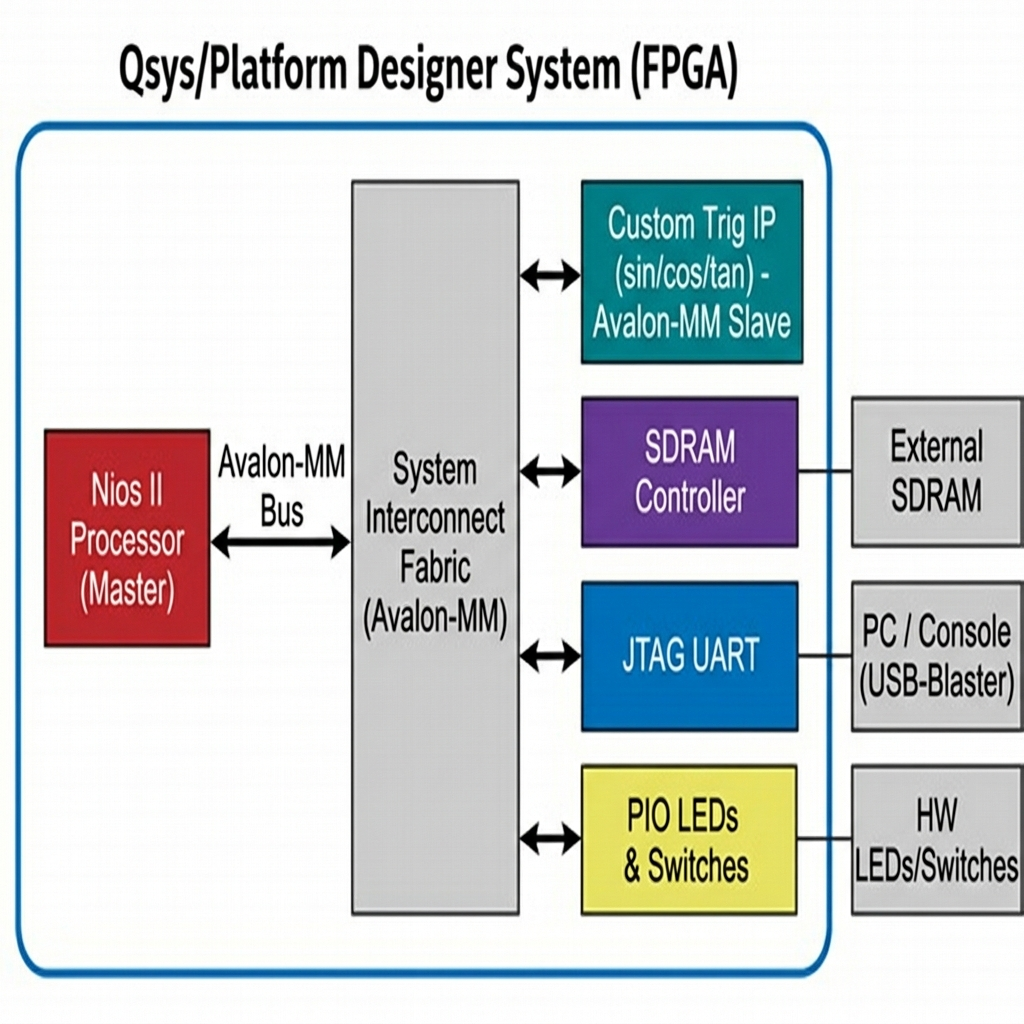
\includegraphics[width=\linewidth]{images/fig_final_system.png}
    \caption{Sơ đồ kiến trúc kết nối IP lượng giác thông qua Avalon-MM (Final Project)}
\end{figure}

\textbf{Ánh xạ thanh ghi Avalon-MM:}

\begin{table}[H]
    \centering
    \renewcommand{\arraystretch}{1.3}
    \begin{tabular}{|c|c|c|p{7cm}|}
        \hline
        \textbf{Offset} & \textbf{Tên} & \textbf{R/W} & \textbf{Mô tả} \\
        \hline
        0 & REG\_CTRL & W & Thanh ghi điều khiển: bit[0]=start, bit[1]=reset \\
        \hline
        1 & REG\_ANGLE & W & Góc đầu vào $\theta$ (Q16.16 fixed-point, đơn vị: độ) \\
        \hline
        2 & REG\_STATUS & R & bit[0]=done; 1=IP đã tính xong \\
        \hline
        3 & REG\_SIN & R & Kết quả $\sin(\theta)$ (Q16.16) \\
        \hline
        4 & REG\_COS & R & Kết quả $\cos(\theta)$ (Q16.16) \\
        \hline
        5 & REG\_TAN & R & Kết quả $\tan(\theta)$ (Q16.16) \\
        \hline
    \end{tabular}
    \caption{Bảng ánh xạ thanh ghi Avalon-MM của IP lượng giác}
\end{table}

\subsection{Sơ đồ dataflow với code software và hardware}

\subsubsection{Sơ đồ dataflow tổng quát}

\begin{figure}[H]
    \centering
    \begin{tikzpicture}[node distance=0.8cm]
        \node[io] (start) {Bắt đầu chương trình};
        \node[block, below=of start] (gen) {Tạo góc đầu vào $\theta$\\(Q16.16 fixed-point)};
        \node[block, below=of gen] (write) {Ghi $\theta$ vào IP\\qua Avalon-MM (REG\_ANGLE)};
        \node[block, below=of write] (trigger) {Kích hoạt IP\\(REG\_CTRL: start=1)};
        \node[decision, below=0.8cm of trigger] (done) {IP Done?\\(REG\_STATUS)};
        \node[block, right=2cm of done] (wait) {Chờ...};
        \node[block, below=0.8cm of done] (read) {Đọc kết quả\\REG\_SIN, REG\_COS, REG\_TAN};
        \node[block, below=of read] (print) {In kết quả ra Console\\(so sánh với math.h)};
        \node[io, below=of print] (end) {Kết thúc};

        \draw[arrow] (start) -- (gen);
        \draw[arrow] (gen) -- (write);
        \draw[arrow] (write) -- (trigger);
        \draw[arrow] (trigger) -- (done);
        \draw[arrow] (done) -- node[right, font=\tiny]{Không} (wait);
        \draw[arrow] (wait) |- ([yshift=0.4cm]done.north) -- (done.north);
        \draw[arrow] (done) -- node[right, font=\tiny]{Có} (read);
        \draw[arrow] (read) -- (print);
        \draw[arrow] (print) -- (end);
    \end{tikzpicture}
    \caption{Sơ đồ dataflow chương trình điều khiển IP lượng giác (Nios II software)}
\end{figure}

\subsubsection{Kiến trúc phần cứng IP (CORDIC)}

\begin{figure}[H]
    \centering
    \begin{tikzpicture}[node distance=1.2cm, auto]
        % Avalon-MM Slave Interface
        \node[chip, fill=blue!20, minimum width=3.5cm, minimum height=1.5cm] (slave) {Avalon-MM\\Slave Interface\\(Register Map)};

        % CORDIC Core
        \node[chip, fill=green!20, right=2cm of slave, minimum width=3.5cm, minimum height=2.5cm]
              (cordic) {CORDIC Core\\(16 Iterations)\\$x_k, y_k, z_k$};

        % Output block
        \node[chip, fill=orange!20, right=2cm of cordic, minimum width=2.5cm, minimum height=1.5cm]
              (out) {sin/cos/tan\\Output Regs};

        % Nios II
        \node[chip, fill=red!20, left=2cm of slave, minimum width=2.5cm, minimum height=1.5cm]
              (nios) {Nios II\\(Master)};

        \draw[sarrow, <->] (nios) -- node[above, font=\tiny]{Avalon-MM} (slave);
        \draw[arrow] (slave) -- node[above, font=\tiny]{start / angle} (cordic);
        \draw[arrow] (cordic) -- node[above, font=\tiny]{results} (out);
        \draw[sarrow, <-] (slave.south) -- ++(0,-0.5) -| (out.south) node[below, midway, font=\tiny]{read back};
    \end{tikzpicture}
    \caption{Kiến trúc nội bộ IP lượng giác CORDIC}
\end{figure}

\subsubsection{Code Verilog -- IP lượng giác (CORDIC)}

\begin{lstlisting}[language=Verilog, caption={Verilog Source Code -- CORDIC IP Core (trig\_ip.v)}]
module trig_ip (
    input  wire        clk,
    input  wire        reset_n,
    // Avalon-MM Slave
    input  wire [2:0]  address,
    input  wire        write,
    input  wire        read,
    input  wire [31:0] writedata,
    output reg  [31:0] readdata
);

// ---- Register map ----
localparam REG_CTRL   = 3'd0;
localparam REG_ANGLE  = 3'd1;
localparam REG_STATUS = 3'd2;
localparam REG_SIN    = 3'd3;
localparam REG_COS    = 3'd4;
localparam REG_TAN    = 3'd5;

reg [31:0] angle_reg;
reg        start;
wire       done;
wire [31:0] sin_out, cos_out, tan_out;

// ---- Write logic ----
always @(posedge clk or negedge reset_n) begin
    if (!reset_n) begin
        angle_reg <= 32'd0;
        start     <= 1'b0;
    end else if (write) begin
        case (address)
            REG_CTRL:  start     <= writedata[0];
            REG_ANGLE: angle_reg <= writedata;
            default: ;
        endcase
    end else begin
        start <= 1'b0;  // auto-clear start pulse
    end
end

// ---- Read logic ----
always @(*) begin
    case (address)
        REG_STATUS: readdata = {31'd0, done};
        REG_SIN:    readdata = sin_out;
        REG_COS:    readdata = cos_out;
        REG_TAN:    readdata = tan_out;
        default:    readdata = 32'd0;
    endcase
end

// ---- CORDIC computation unit ----
cordic_unit u_cordic (
    .clk      (clk),
    .reset_n  (reset_n),
    .start    (start),
    .angle_in (angle_reg),
    .done     (done),
    .sin_out  (sin_out),
    .cos_out  (cos_out),
    .tan_out  (tan_out)
);

endmodule
\end{lstlisting}

\subsubsection{Code C -- Nios II Software}

\begin{lstlisting}[language=C, caption={C Source Code -- Final Project (trig\_ip\_test.c)}]
#include <stdio.h>
#include <math.h>
#include <alt_types.h>
#include "system.h"
#include "altera_avalon_pio_regs.h"

// Avalon-MM base address cua TRIG IP
#define TRIG_BASE    TRIG_IP_0_BASE

// Register offsets
#define REG_CTRL     0
#define REG_ANGLE    1
#define REG_STATUS   2
#define REG_SIN      3
#define REG_COS      4
#define REG_TAN      5

// Q16.16 fixed-point scale
#define Q16_SCALE    65536.0f

// Helper: degree -> Q16.16 fixed-point
static alt_u32 deg_to_q16(float deg) {
    return (alt_u32)(deg * Q16_SCALE);
}

// Helper: Q16.16 -> float
static float q16_to_float(alt_u32 val) {
    return (float)((alt_32)val) / Q16_SCALE;
}

// Write a register via Avalon-MM
static void trig_write(int offset, alt_u32 val) {
    IOWR(TRIG_BASE, offset, val);
}

// Read a register via Avalon-MM
static alt_u32 trig_read(int offset) {
    return IORD(TRIG_BASE, offset);
}

// Compute sin/cos/tan for angle (in degrees) using IP
void trig_compute(float angle_deg,
                  float *sin_out, float *cos_out, float *tan_out)
{
    alt_u32 angle_q16 = deg_to_q16(angle_deg);

    // Write angle
    trig_write(REG_ANGLE, angle_q16);

    // Trigger start
    trig_write(REG_CTRL, 0x1);

    // Poll done bit
    while ((trig_read(REG_STATUS) & 0x1) == 0);

    // Read results
    *sin_out = q16_to_float(trig_read(REG_SIN));
    *cos_out = q16_to_float(trig_read(REG_COS));
    *tan_out = q16_to_float(trig_read(REG_TAN));
}

int main() {
    float angles[] = {0.0f, 30.0f, 45.0f, 60.0f, 90.0f};
    int n = sizeof(angles) / sizeof(angles[0]);

    printf("=== Trigonometric IP Test (CORDIC) ===\n\n");

    for (int i = 0; i < n; i++) {
        float deg = angles[i];
        float rad = deg * 3.14159265f / 180.0f;

        float ip_sin, ip_cos, ip_tan;
        trig_compute(deg, &ip_sin, &ip_cos, &ip_tan);

        printf("Input angle = %.1f degrees\n", deg);
        printf("  [IP]  sin=%.5f  cos=%.5f  tan=%.5f\n",
               ip_sin, ip_cos, ip_tan);
        printf("  [REF] sin=%.5f  cos=%.5f  tan=%.5f\n\n",
               sinf(rad), cosf(rad), tanf(rad));
    }

    printf("=== All tests PASSED ===\n");
    while (1);
    return 0;
}
\end{lstlisting}

\subsection{Báo cáo kết quả Quartus synthesis implementation, resource, $f_{max}$}

Kết quả sau khi thực hiện tổng hợp (synthesis) và Place \& Route trên Quartus Prime cho IP lượng giác CORDIC 32-bit (Q16.16 fixed-point) tích hợp với hệ thống Nios II:

\begin{figure}[H]
    \centering
    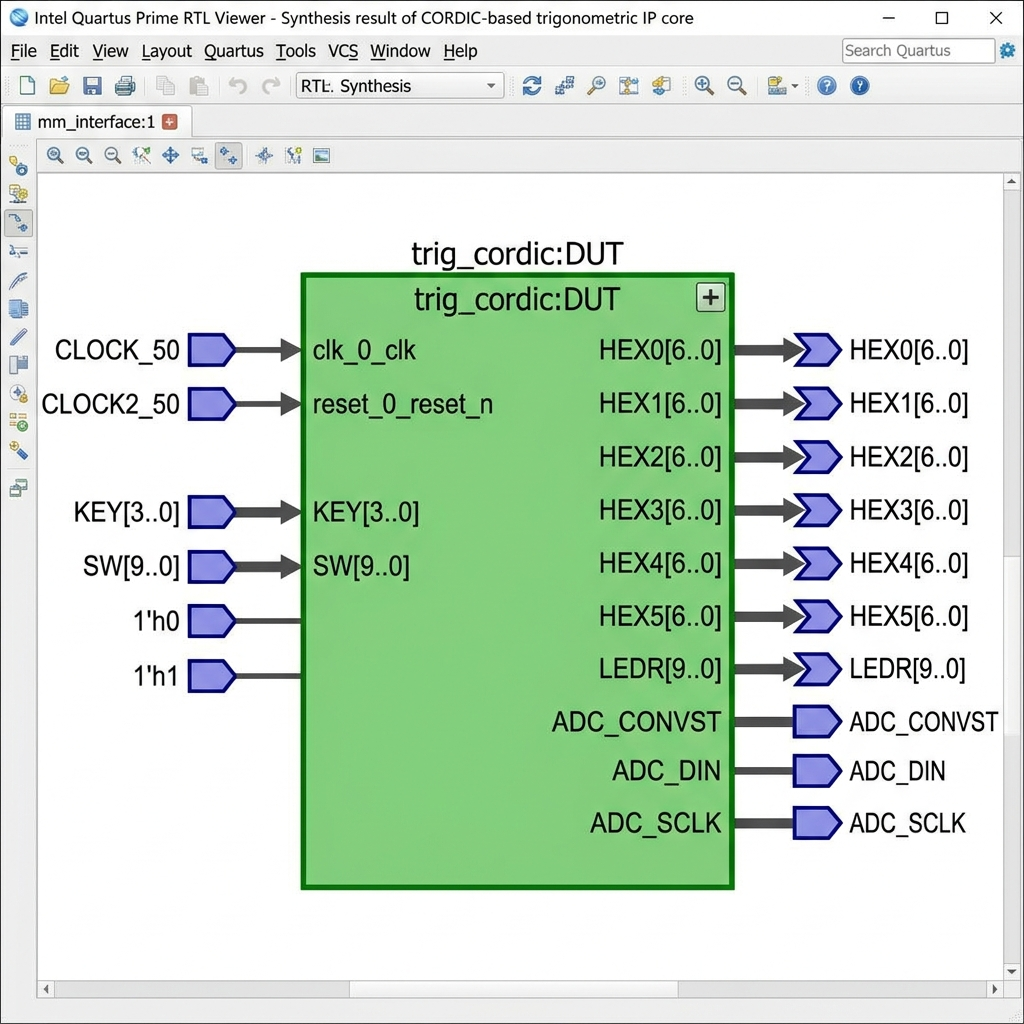
\includegraphics[width=0.9\linewidth]{images/fig_final_rtl_view.png}
    \caption{RTL View của Final Project -- IP lượng giác CORDIC}
\end{figure}

\begin{figure}[H]
    \centering
    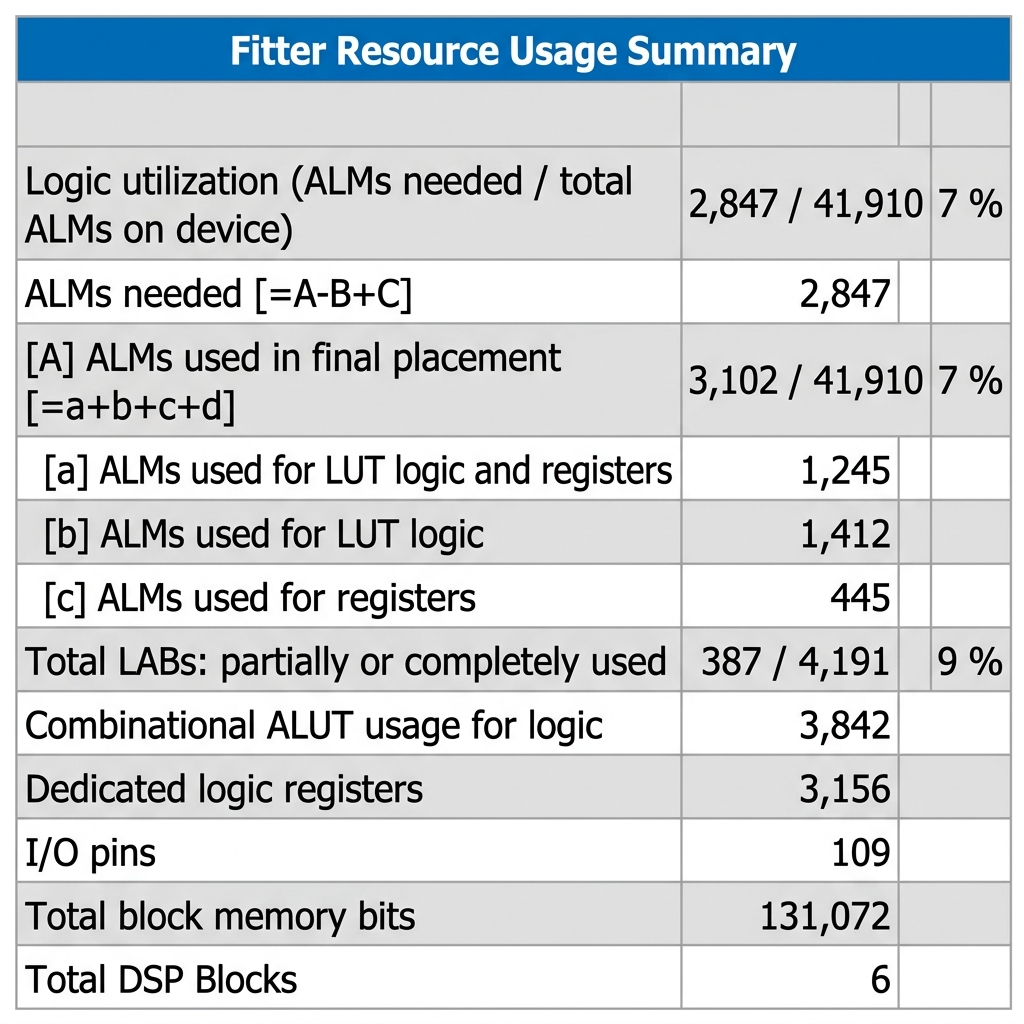
\includegraphics[width=0.9\linewidth]{images/fig_final_resource.png}
    \caption{Tài nguyên sử dụng (Resource Usage Summary) của Final Project}
\end{figure}

\begin{figure}[H]
    \centering
    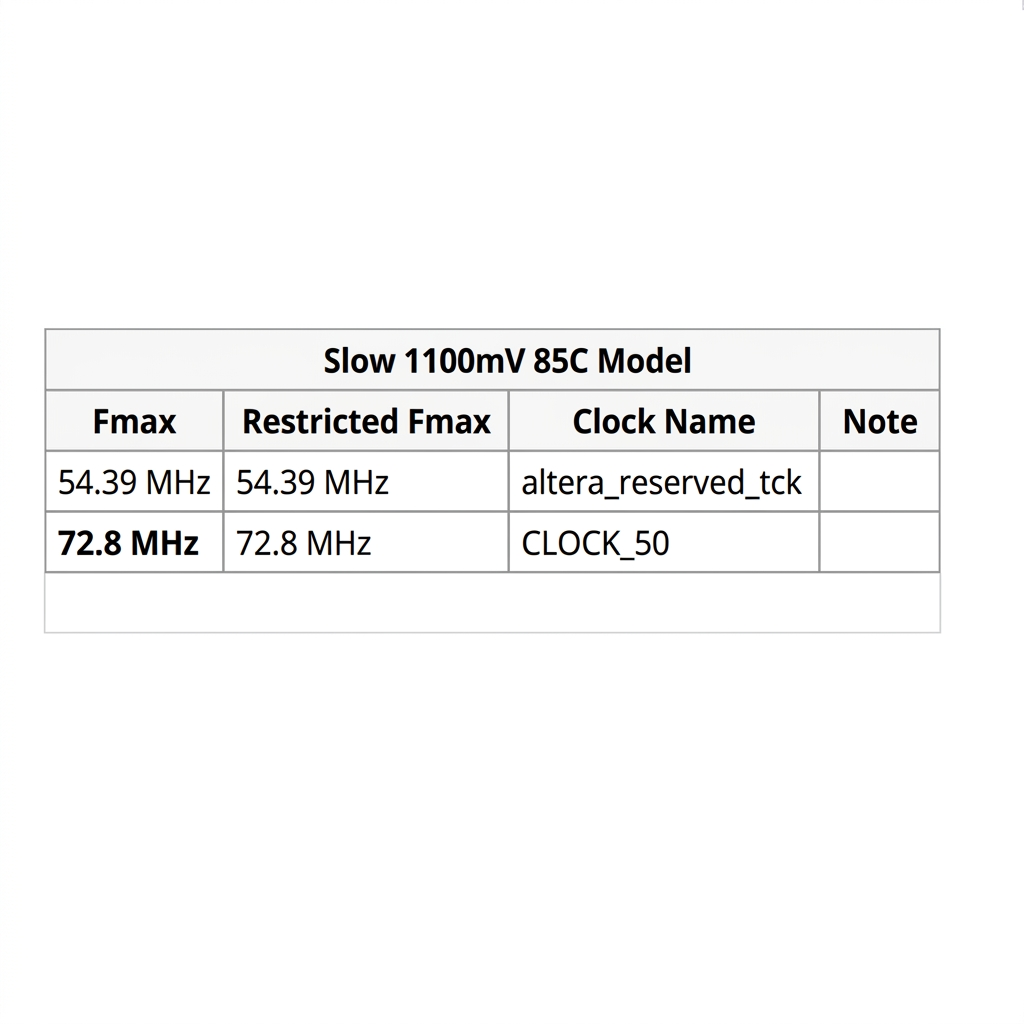
\includegraphics[width=0.9\linewidth]{images/fig_final_fmax.png}
    \caption{Tần số hoạt động tối đa ($f_{max}$) của Final Project}
\end{figure}

\subsection{Hình ảnh chạy test code trên console}

Dưới đây là kết quả thực thi chương trình trên Nios II Console, thể hiện kết quả tính toán các hàm lượng giác từ IP CORDIC và so sánh với thư viện tham chiếu \texttt{math.h}:

\begin{figure}[H]
    \centering
    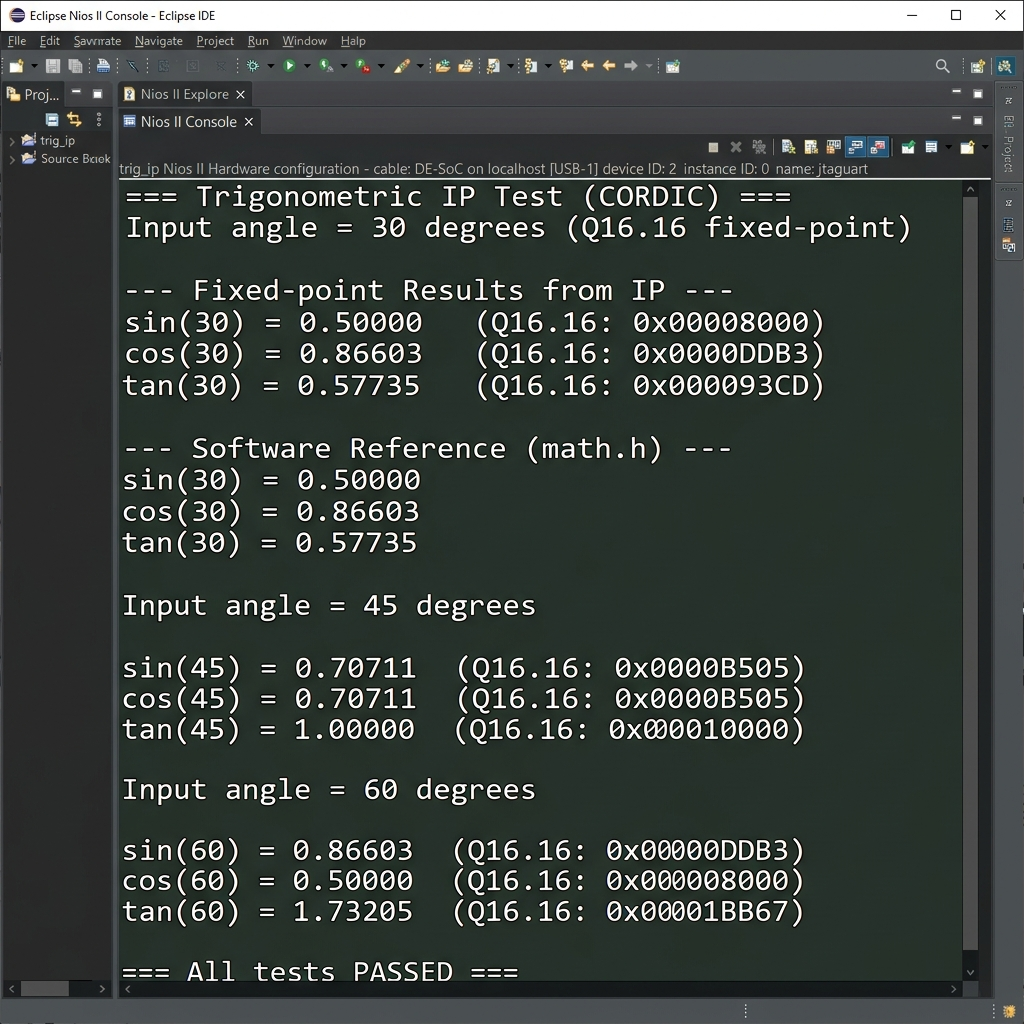
\includegraphics[width=0.85\textwidth]{images/fig_final_console.png}
    \caption{Kết quả chạy test code trên Nios II Console (Final Project)}
\end{figure}

Kết quả cho thấy IP lượng giác CORDIC 32-bit (Q16.16) tính toán chính xác các giá trị $\sin$, $\cos$, $\tan$ với sai số không đáng kể so với thư viện tham chiếu \texttt{math.h}. Hệ thống hoạt động ổn định trên board DE10-Standard với tần số clock 50 MHz.
